The literature review identified 3 general paths that one could take when developing a classifier, each with a different
set of strengths, weaknesses, and aiming to address different priorities.
The following sections will discuss the approaches taken to develop the three models to be evaluated further, in an
increasing order of complexity.
\section{Nearest-neighbor classifier}
\label{sec:knn-classifier}
The primary reasoning behind implementing a KNN-based classifier is its speed of deployment, simplicity of implementation
and good accuracy potential.
As a concept, KNN can be easily understood even by non-technical stakeholders and requires little experimentation apart
from picking the value of K, determining how many ''neighbors`` each input has to be compared against.

One of the main challenges with KNN is its computational cost: the number of comparisons grows quickly with an increase
in the amount of features, dimensions and data points.
Therefore, with the dataset's images containing tens of thousands of pixels, each with three colour channels, a brute-force
approach was dismissed.

An approach seen, among others, in Olivieri et. al.'s paper~\cite{hyperspectralGreenOliveri}, is dimensionality reduction,
which aims to extract the features of the data that contribute to its difference the most.
While several dimensionality reduction techniques exist, the significant visual differences across the bean classes suggested
that the use of colour histograms could efficiently reduce the size of the data while still preserving its differences.

A colour histogram is a relatively simple plot of the distribution of colours in a given image.
A strength of this approach is its resilience to the orientations of beans in the images - the colour distribution stays
the same no matter how the bean is positioned (apart from the small discrepancies in shadows).
Furthermore, the dimensionality of the resulting data can be adjusted by changing the number of bins in the diagram, allowing
the representation to be more or less precise depending on the task.
An example of such histogram is shown on figure~\ref{fig:histExample}.

\begin{figure}[h]
    \centering
    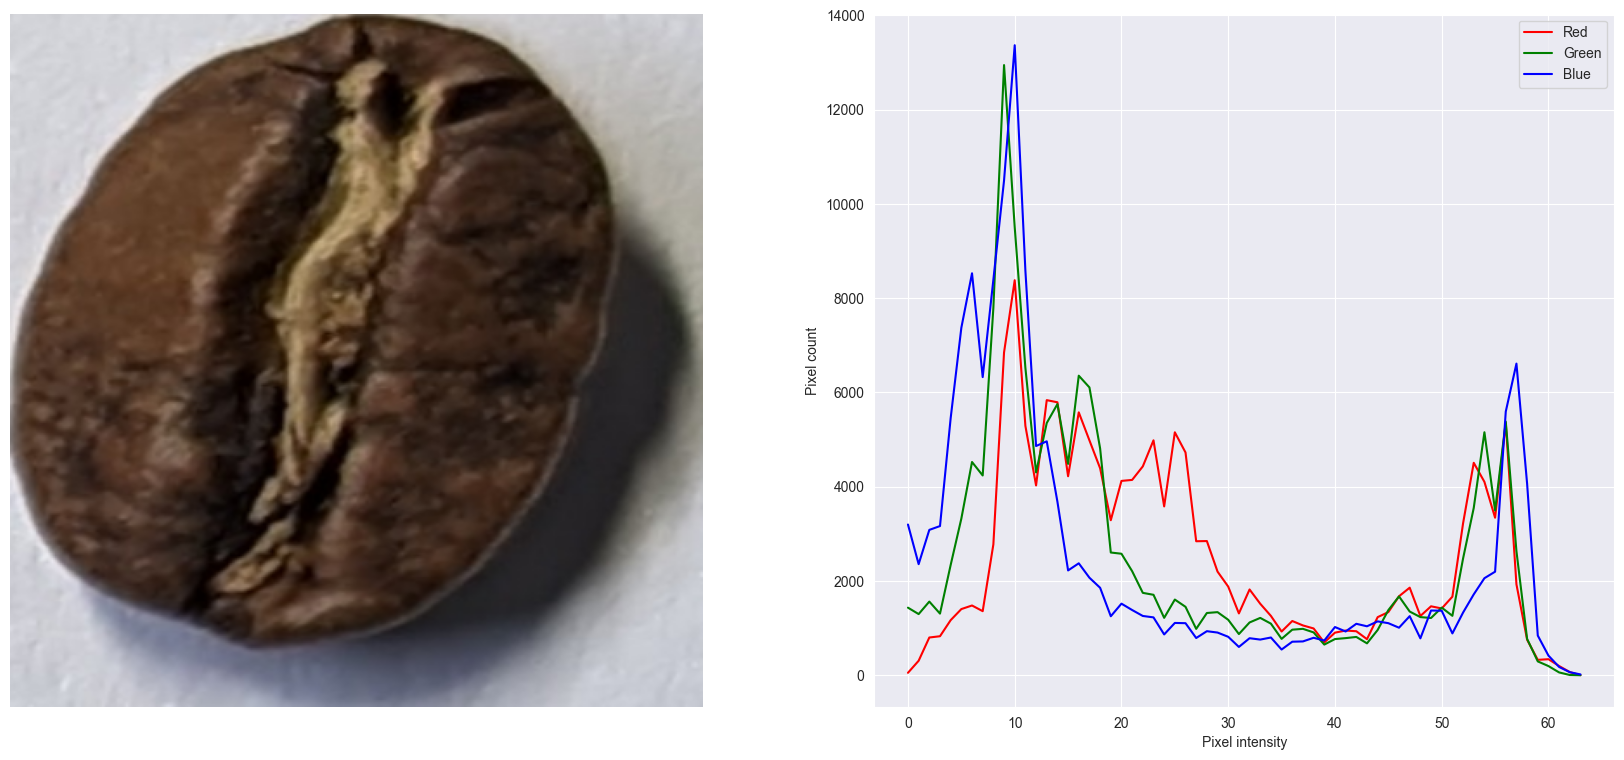
\includegraphics[height=4cm, keepaspectratio]{figures/methodology/histogramExample}
    \caption[Colour histogram example]{A colour histogram example (64 bins)}
    \label{fig:histExample}
\end{figure}
Placing each curve ''side-by-side`` allows for an image to be represented by a vector of length $nbins \times nchannels$,
where $nbins$ and $nchannels$ represent the number of histogram bins and the number of colour channels in an image respectively.

It should be noted that the method is not without its criticisms: while colour makes up a significant amount of the difference
between the beans, properties like texture and shape are removed by the dimensionality reduction process.
Also, the size of the image itself can skew the distribution simply due to the difference in the numbers of pixels if the
images are not resized prior to histogram calculations.

Another approach to a KNN classifier was tested in a preliminary experiment:
there, the images were converted into long vectors by extracting colour information from each channel (red, green or blue)
and concatenating the three resulting grids into a one-dimensional representation.
While this approach was able to correctly classify some images, especially those belonging to the ''normal`` and ''quaker``
classes, the performance on the smaller classes combined with the long prediction times suggested that the colour histogram
provided a better compromise between the richness of the data and the practicality of the classifier.

The best hyperparameters were found in a grid search, with different choices of the value of k, the distance metric
and nearest neighbour calculation algorithm trialed.
In every experiment, the classifier was fitted with 80\% of the data, chosen at random and evaluated on the rest of the data,
with metrics such as overall accuracy, per-class precision, recall and f1 score recorded and tracked.
To maintain a consistent ratio of beans of different types, a stratified split function has been used.

The classifiers and their evaluation were implemented using the Scikit-learn library \cite{sklearnLibrary}, with the calculation of colour
distributions provided by the Scikit-image library~\cite{skImageLibrary}.
Loading the data was done by creating a \verb|DataLoader| class provided by the PyTorch library \cite{pytorchLibrary}, which allowed
for the data loading to be easily shared between this classifier and ones developed later.
\section{Compact CNN classifier}
\label{sec:deep-learning}
The aims in developing this classifier were centered around addressing the weaknesses of the one described above,
namely its high prediction cost and its lack of ability to extract complex features from input images.

For this, a convolutional neural network (CNN) was selected as a design candidate, based on their
efficiency at classifying images and common use in industry.
Furthermore, the principles behind the functionality of convolution layers suggest that the high resolution of the input
images would be a benefit, with the classifier being able to extract texture and shape information from each image.

While countless network architectures exist, the goal with this classifier was ensuring the smallest possible classification time,
and, therefore, smaller designs were considered.
The MobileNet V2 architecture~\cite{mobileNet} stood out for its relatively small number of parameters and a promised ability to run even on
a mobile device.


\begin{wrapfigure}{r}{0.4\textwidth}
    \centering
    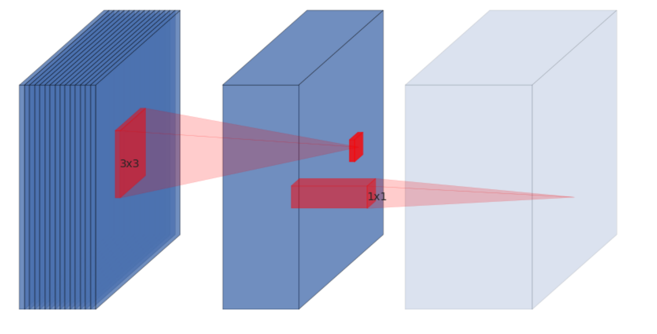
\includegraphics[width=0.4\textwidth]{methodology/depthwise-conv}
    \caption[Depthwise convolution]{Depthwise convolution~\cite{mobileNet}}
    \label{fig:depthwiseConv}
    \vspace{-1em}
\end{wrapfigure}

Such a small size has been achieved by the authors' usage of depthwise convolution layers seen on figure~\ref{fig:depthwiseConv},
where a ''traditional`` convolution block is split into two stages: first, each channel is processed separately with a $1 \times W \times H$ filter.
Then, the resulting intermediate representation is consolidated using a $nChannels \times 1 \times 1$ filter.
Doing so still allows the network to learn the relationships between channels and achieve high benchmark results, with the models requiring
a fraction of the number of parameters of conventional CNN's~\cite{mobileNet}.
Achieving a high performance result from such a small architecture would result in a classifier that is able to be deployed
on any system, removing the cost barrier between coffee roasters and automatic quality control methods.
Furthermore, a smaller architecture would be faster to train on a custom dataset, providing greater flexibility.

Other smaller architectures such as ShuffleNet V2`~\cite{shuffleNet} were considered and trialled in preliminary experiments,
however, MobileNet consistently outperformed the others and was therefore selected as the best performer of this section.
\section{Application of transfer learning to large models}
\label{sec:transfer-learning}
The models trialled in this set of experiments were the largest in terms of the number of parameters and
architectural complexity.
The idea behind using these models was that the large number of parameters could allow them to extract even more information
from the input images and gain better performance, especially in smaller classes.

A drawback of such large modules is their need for large dataset during training, a requirement which the gathered data would
struggle to fulfil.
To overcome this limitation, a technique called transfer learning was employed.
In this technique, the model is first trained on a large, not necessarily domain-specific dataset and then
''fine-tuned`` on a smaller selection of domain-specific data.
This technique allows the models to learn to extract features from images and then sharpen that knowledge by training on a dataset
specific to the given task.

A commonly used general-purpose dataset is ImageNet~\cite{imageNet}, containing over a million images belonging to a thousand
classes.
Pre-trained models were loaded from the \verb|torchvision.models| package provided by PyTorch~\cite{pytorchLibrary}.

One of the more promising architectures was ResNet~\cite{resNet}, with a deep architecture boasting a high top-1 accuracy on the imageNet dataset.
Several versions of the ResNet architecture exist, with the 18, 34 and 50 layer versions trialled in the experiments.
\newline
\begin{wrapfigure}{r}{0.4\textwidth}
    \centering
    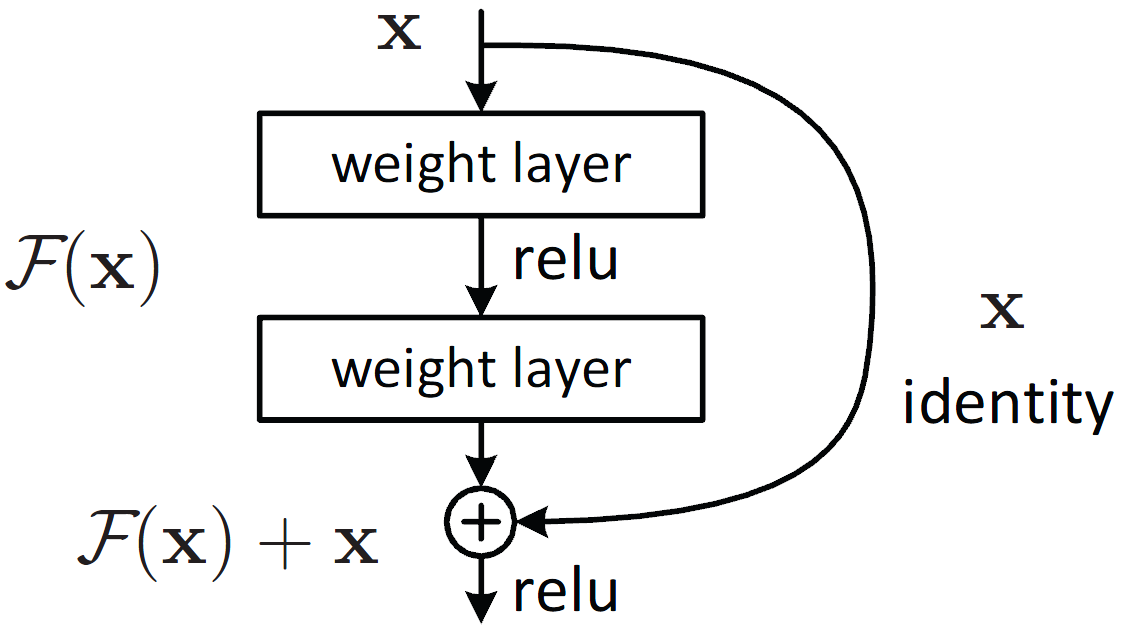
\includegraphics[width=0.4\textwidth]{methodology/residual-block}
    \caption[Residual block]{Residual block~\cite{resNet}}
    \label{fig:residualBlock}
\end{wrapfigure}
The main innovation behind this family of classifiers is their use of ''residual blocks`` (with an example shown on figure~\ref{fig:residualBlock}), an architecture where the output of
a chain of convolution layers is added to the input and passed along further rather than just the output being passed on.
This architecture choice has led to improvements on ImageNet performance, and remains the state-of-the-art in image classification.
By having access to both the unmodified input and the output of the convolution layers, it is possible to make use of both representations,
leading to better accuracy~\cite{resNet}.

Other tested architectures included the EfficientNet V2~\cite{efficientNet} and the Swin transformer~\cite{swinTransformer},
which were selected for their reported accuracy on the imageNet dataset.

An important step in this set of experiments was the readjusting of the model before making predictions on the bean dataset:
since all models were tailored to ImageNet, the number of output neurons in their final fully-connected layers was mismatched.
The fixes involved inspecting the models' architectures, identifying the attribute name of the final layer, and replacing it with an
instance of the \verb|torch.nn.Linear()| class, where the number of input neurons matched that of the old fully connected layer,
and the number of outputs was equal to the number of classes in the dataset.